\section{Greedy Algorithm}

    A greedy algorithm always makes the choice that looks best at the moment.
    That is , it makes a locally optimal choice in the hope that this choice
    will lead to a globally optimal solution.

\subsection{An activity-selection problem}

    Suppose we have a set $S=\lbrace a_1,a_2,...,a_n \rbrace$
    of n proposed activities that wish to use a resource, 
    such as a lecture hall, which
    can serve only one activity at a time.

    Each activity $a_i$ has a start time $s_i$ and a finish time $f_i$,
    where $0\leq s_i \leq f_i \leq \inf$. $a_i$ and $a_j$ are 
    compatible if $s_i > f_j$ or $s_j > f_i$.

    In the activity-selection problem, we wish to select a maximum-size
    subset of mutually compatible activities.

    Assume that the activities are sorted in increasing order of finish time
    \begin{equation*}
        f_1 \leq f_2 \leq f_3 ... f_{n-1} \leq f_n
    \end{equation*}

    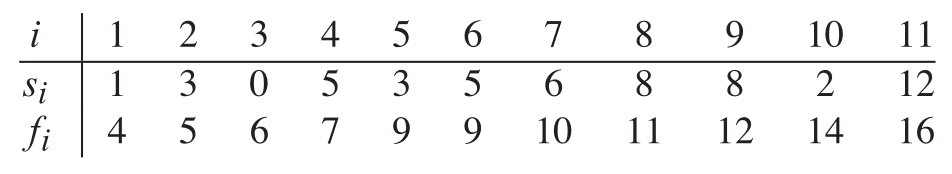
\includegraphics[width=0.4\textwidth]{contents/Advanced_Design/Greedy/greedy_image/sorted_finish_time.png}


    The approach is try to solve with dynamic programming and observe that 
    only one choice should be consider - the greedy choice, that is 
    DP with one subproblem.

    Let c[i,j] denoted the maximum size of an optimal solution for set $S_{ij}$.
    $S_{ij}=\lbrace a_k: f_i \leq s_k \leq f_k \leq s_j  \rbrace$.

    The reccurence of choosing $a_k$

    \begin{equation*}
        c[i,j] = c[i,k] + c[k,j] + 1
    \end{equation*}

    \[ c[i,j]= \begin{cases} 
        0 & \text{if } S_{ij}=\emptyset \\
        max_{a_k \in S_{ij}} \lbrace c[i,k]+c[k,j]+1 \rbrace &
        \text{if } S_{ij} \neq \emptyset
     \end{cases}
    \]
  
\subsubsection*{Making the greedy choice}


    Intuition suggests that we should choose an activity that leaves the resource available
    for as many other activities as possible: choose the earliest finish time.

    By choosing "the" activity, we only left one subproblem.
    
    Let $S_k = \lbrace a_i \in S: s_i \geq f_k \rbrace$ be the set of activities
    that start after $a_k$ finishes.

    But why is the intuition correct?

    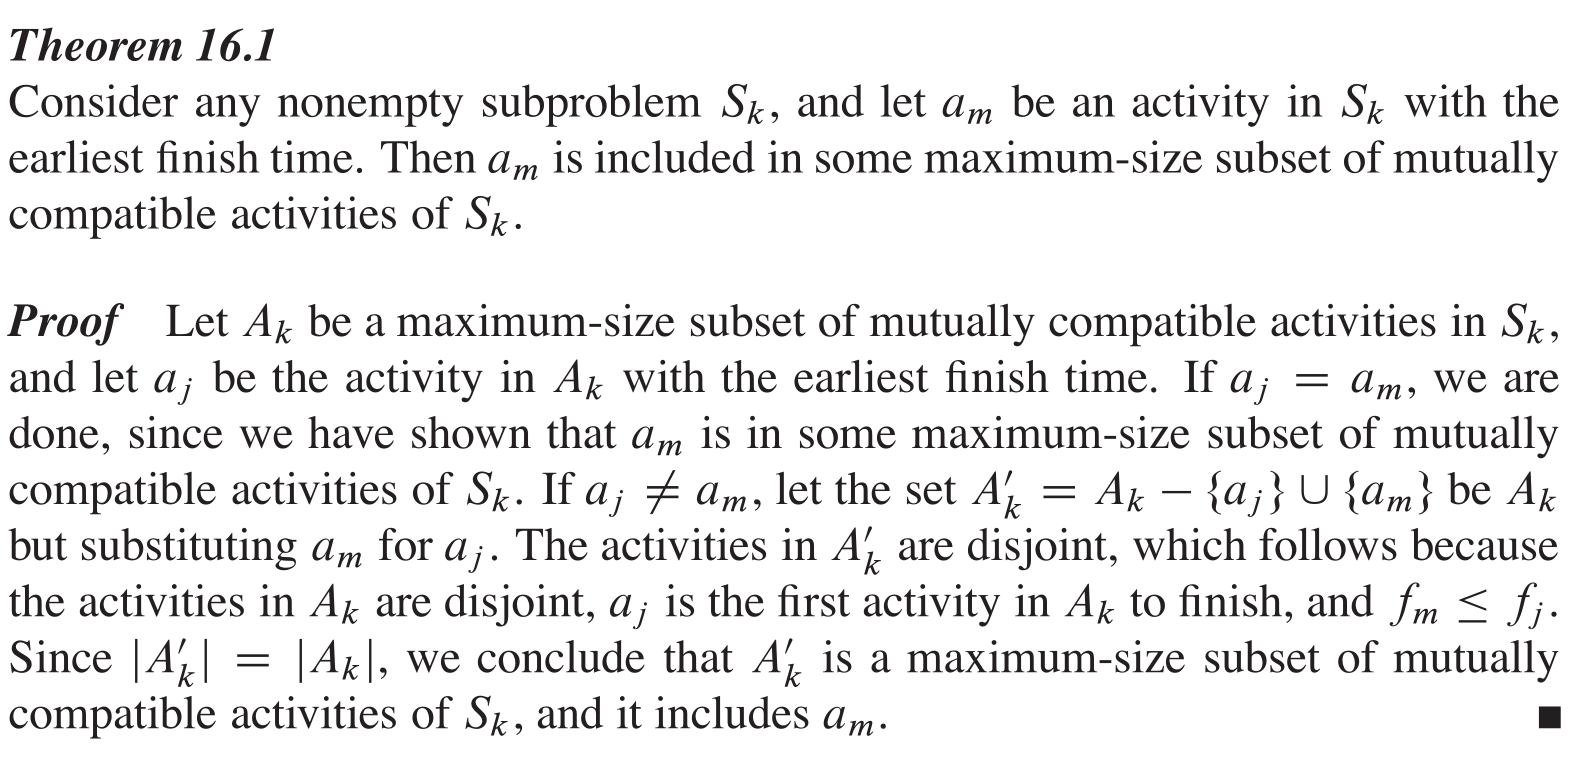
\includegraphics[width=0.6\textwidth]{contents/Advanced_Design/Greedy/greedy_image/proof_earliest_finish_time.png}

    Greedy algorithms typically have this top-down design: make a
    choice and then solve a subproblem, 
    rather than the bottom-up technique of solving
    subproblems before making a choice.


\subsubsection*{A recursive greedy algorithm}

     Assume that the n input activities are already ordered 
     by monotonically increasing finish time.

     In order to start, we add the fictitious 
     activity a0 with $f_0=0$, so that subproblem $S_0$ is
    the entire set of activities S.

    \begin{lstlisting}
        RECURSIVE-ACTIVITY-SELECTOR(s,f,k,n)
        {
            // select the earliest finish time activity
            int m = k+1;
            // such that s_m >= f_k (k is the last choice)
            while( m <= n && s[m] < f[k])
            {
                m = m+1;
            }

            if(m <= n)
            {
                // subproblem, maximum mutable compatible set of S_m
                return union(a_m,RECURSIVE-ACTIVITY-SELECTOR(s,f,m,n));
            }

            return []
        }
    \end{lstlisting}


    \textbf{Time Complexity:} O(n) which is very obvious.

\subsubsection*{An iterative greedy algorithm}

    \begin{lstlisting}
        GREEDY-ACTIVITY-SELECTOR(s,f)
        {
            int n = s.length;
            A = [a1];
            int k = 1;
            for(int m=1; m<n; m++)
            {
                if s[m] > f[k]
                {
                    A.append(a_m);
                    k = m;
                }
            }

            return A;
        }
    \end{lstlisting}



\subsection{Elements of the greedy strategy}

    The greedy strategy doesn't always yield an optimal solution.

    In order to use greedy method:
    \begin{enumerate}
        \item Determine the optimal substructure of the problem.
        \item Develop a recursive solution.
        \item Show that if we make the greedy choice, then only one subproblem
        remains.
        \item Prove that it is always safe to make the greedy choice.
        \item Develop a recursive algorithm that implements the greedy strategy.
        \item Convert the recursive algorithm to iterative algorithm.
    \end{enumerate}

    In the activity-selection problem, we proved that a greedy
    choice (the earliest finish time $a_m$ to finish in $S_k$), combined 
    with an optimal solution to the reaming $S_m$ of compatible activities,
    yields an optimal solution to $S_k$.
   
    More generally,
    \begin{enumerate}
        \item Think the optimization is to make a choice and solve the 
        remaining subproblem.
        \item Prove that there is always an optimal solution to the original
        problem that makes greedy choice $\Leftrightarrow$ the greedy
        choice is always safe.
        \item Demonstrate optimal substructure by showing that, having
        made the greedy choice, what remains is a subproblem with the property
        that if we combine an optimal solution to the subproblem with 
        the greedy choice, we arrive at an optimal solution to the original 
        problem.
    \end{enumerate}

    \subsubsection*{Greedy-choice property}

    
























